\section{Experimental Setup}
\label{sec:exp-setup}

\cmtDK[inline]{15 pages}
\cmtDK[inline]{\\
    - what is ambiguity? \\
    - unambigous dataset: \\
    ---- target group = non-target group \\
    ---- all attributes shared, except for the color \\
    ---- \ \  --> describable with one 'word'
}
In this section I will describe which experiments were conducted to answer the \cmtDK{?}{questions} from the previous sections as well as the setup of these experiments.
This will be done in two parts.
The first part contains the creation of the datasets that will be used in the experiments.
In the second part I will go deeper into discussing each experiment, including the necessity of the experiment, the specifities of the dataset, as well as the final architecture of the models.

\subsection{Creation of the dataset}
The basis for my dataset is the CLEVR dataset (\cite{Johnson2016}).
This dataset includes 3D-generated images depicting scenes with different kind of objects.
Each of these objects has different combinations attributes, such as \emph{shape}, \emph{color}, \emph{size} and \emph{material}.
The possible values of these attributes are listed in Table \ref{tab:clevr-attributes}.
Three to ten objects are randomly placed into the scene and assigned with random attributes.
To enhance realism and reduce ambiguity, objects do not intersect, have a certain distance from each other, and are at least partially visible.
Figure \ref{fig:clevr-example} shows an example of a generated image in the CLEVR dataset.

\begin{table}[h]
    \centering
    \begin{tabular}{cccc}
        \toprule
        \textbf{ shape } & \textbf{ color } & \textbf{ size } & \textbf{ material } \\
        cube             & gray             & small           & rubber              \\
        sphere           & red              & large           & metal               \\
        cylinder         & blue                                                     \\
                         & green                                                    \\
                         & brown                                                    \\
                         & purple                                                   \\
                         & cyan                                                     \\
                         & yellow                                                   \\
        \bottomrule
    \end{tabular}
    \caption{Attributes of objects in the CLEVR dataset}
    \label{tab:clevr-attributes}
\end{table}

\begin{figure}[h]
    \centering
    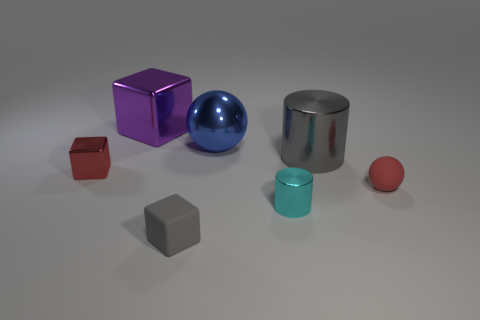
\includegraphics[width=.8\linewidth]{figures/CLEVR_example.png}
    \caption{Example of a generated image in the CLEVR dataset}
    \label{fig:clevr-example}
\end{figure}

Furthermore, the dataset contains information about each scene.
This includes the selected attributes for each object as well as the exact position of the centers of all the objects, both 3D-coordinates in the 3D scene and 2D-coordinates in the final rendered image.
In addition, simple spatial relations (in front of, behind, left, right) between the objects are calculated and stored.
These are simply based on the 3D-coordinates of the objects from the perspective of the camera position.

\cmtDK[inline]{ambiguity}

This research investigates how agents communicate about the relations of objects seen in images.
For that reason the original CLEVR dataset offers too little control over how the objects are created and in which relation they stand to each other.
Following, I extended the source code to generated images for the CLEVR dataset.\footnote{\href{https://github.com/DominikKuenkele/MLT\_Master-Thesis\_clevr-dataset-gen}{https://github.com/DominikKuenkele/MLT\_Master-Thesis\_clevr-dataset-gen}}
To simplify the generation, I only focused on the attributes \emph{shape}, \emph{size} and \emph{color}.
The \emph{material} is always the same for all objects in a generated image.
There were three main extensions to the code:

First, objects in the scene were separated into three categories: one \emph{target object}, objects in a \emph{target group} and \emph{distractor} objects.
The target object is the main object in the scene that should be identified and communicated by the agents.
All other objects and their relations are based on this target object.
The target group contains similar objects to the target object.
These are objects that the agents need to discriminate the target object from.
Finally, the distractors are objects that add noise to the scene and should make it more complex and are expected to teach the agents more precise descriptions.
The number of the objects in both group can be controlled.

In a second step, when generating the images it is possible to define the relations between \emph{target object}/\emph{target group} and \emph{target object}/\emph{distractors}.
The relation is defined as \textbf{how many} attributes of the target object are identical with objects in the target group and distractors respectively.
For example the target object is a \emph{small red cube}.
If two attributes are shared between target object and target group, objects in the target group could include \emph{small blue cube}, \emph{big red cube} or \emph{small red sphere} but couldn't include another \emph{small red cube} or a \emph{small blue cylinder}.
The number of shared attributes can also be set to a range to make the discrimination task more challenging.

Lastly, it is also possible to define exactly \textbf{which} attributes should be shared between the target object and the groups.
For example, it can be defined to have the same size for objects in the target group, but have randomly selected different shapes and color.
This allows a very controlled generation of relations between the objects in the scene.
Figure \ref{fig:clevr-extended_example} shows one generated image with this extended source code.
Here, the target object is the large purple cylinder.
The target group contains four objects that share zero to a maximum of two attributes.
It is not controlled, which attributes are shared (they are selected randomly).
There are no distractor objects.

\begin{figure}[h]
    \centering
    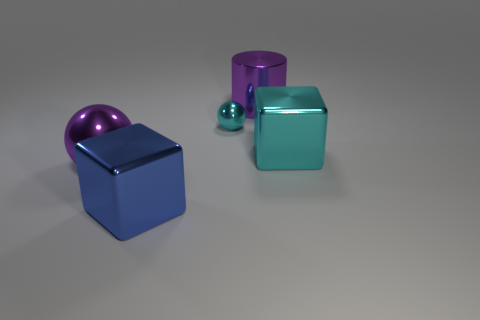
\includegraphics[width=.8\linewidth]{figures/CLEVR_extended_example.png}
    \caption{Example of a generated image with the extended code}
    \label{fig:clevr-extended_example}
\end{figure}

For all generated datasets in the following sections, the general constraints and settings are as close as possible to the original CLEVR dataset.
The size of the generated images is 480x320 pixels.
10.000 images are created for each of the datasets.
Each image contains a maximum of 10 objects, that are not intersecting, have the same minimum distance and are partially visible.

\subsection{Description of experiments}
Language games are very complex setups for machine learning models.
The models need to solve multiple tasks at the same time to solve the overall problem.
For instance in a simple setup of a game two agents are involved.
The first agent, the sender is shown a scene with objects and needs to communicate on target object to the other agent, the receiver.
The receiver is shown the same scene and needs to identify the target object with respect to the message of the sender.
In this case, the sender first needs to learn to encode the scene as well as the information about the target object into its own \cmtDK{?}{space}.
In a next step it needs to learn how to translate this encoding into a message that is sent to the receiver.
The receiver then needs to learn to decode this message, after which it needs to learn how to combine the decoded message with its own encoding of the scene.
And finally it needs to learn how to identify the target object with this information.

For this reason I decided to divide the main problem and let the models learn simpler subtasks and increase the complexity step by step.
This will give me a very detailed overview, where the models struggle to learn and in which ways they can be improved.
Mainly, I separated the tasks into language games with two agents (final experiments) and classical machine learning tasks without any communication, namely only one 'agent' that solves the task alone (pre-experiments).
With this division, I can analyze the learning of the encodings of the scenes separately from the learning of producing and decoding messages.

\subsubsection{Pre-experiments without language games}
The final objective of this thesis is to find out, how agents can communicate about relations of objects spatially as well as based on their attributes.
Because of that, the first experiments focus on extracting information from images and combining them with structured knowledge.
Here, I structured the experiments into three levels.
In the first level, the model are trained to learn the position of objects in the image and attend to specific regions of the image.
In the second level, the models are trained to differentiate objects in the image from each other.
The last level adds language to the experiment, more specifically the models learn to caption and describe objects in and image.
These combined experiments should lay the basis for how to build up the agents in the language games.

\paragraph{coordinate predictor}
\cmtDK[inline]{talk about why coordinates are necessary for language games}
\cmtDK[inline]{\\
    - pretrained ResNet/VGG\\
    - scratch \\
    - encoding of attributes (one-hot) \\
    - encoding of attributes (dale) \\
    - encoding of locations \\
    - masking}

For these experiments, the model is trained to predict the location of an object for a given image.
In the simplest setup, the model receives only the image as an input and produces two numbers as an output, the predicted x- and y-coordinate of the target object.
Here the image is first passed through a \emph{feature extractor}.
These feature extractors are a deep neural model that are designed to extract important information from images.
Here, I chose ResNet (\cite{He2016}) and VGG (\cite{Simonyan2015}) as a basis.
Both of those models can be used with pretrained weights, trained on classifying images from big datasets.
Since these pretrained weights are based on a very different task than in this thesis, I experimented with different architectures of these feature extractors.
Namely, I used both VGG19 and ResNet101 with random initializations and pretrained on the classifying task.
Furthermore, I removed and/or replaced the last layers of either network.
The idea behind this was, that \cmtDK{cite}{the models learn more general features in the first layers, while the last layers are fine-tuned more specifically to this task.}

\paragraph{bounding box classifier}

\paragraph{caption generator}
\cmtDK[inline]{\\
    - dale \\
    - masked}

\subsubsection{Language games}